\chapter{User Personas: Problem 3}
\vspace{6pt}

\section{Definition}
\vspace{4pt}
\noindent
Persona gives meaningful archetypes which we can use to assess our design development against. 
Personas are actually fictional characters, which we create based upon our research in order to represent the different user types that might use our service, product, site, or brand in a similar way. Creating personas will help us to understand our users’ needs, experiences, behaviors and goals.

\\
\vspace{4pt}
\noindent
\begin{flushleft} 

Constructing personas will help us ask the right questions and answer those questions in line with the users we are designing for. Creating personas can help we step out of ourselves. It can help us to recognize that different people have different needs and expectations, and it can also help us to identify with the user we’re designing for. Personas make the design task at hand less complex, they guide our idea processes, and they can help we to achieve the goal of creating a good user experience for our target user group.
\end{flushleft} 
\\
\vspace{4pt}
\noindent
\begin{flushleft} 
As opposed to designing products, services, and solutions based upon the preferences of the design team, it has become standard practice within many human centered design disciplines to collate research and personify certain trends and patterns in the data as personas. Hence, personas do not describe real people, but we compose our personas based on real data collected from multiple individuals. Personas add the human touch to what would largely remain cold facts in our research. When we create persona profiles of typical or atypical (extreme) users, it will help we to understand patterns in our research, which synthesizes the types of people we seek to design for. Personas are also known as model characters or composite characters.
\end{flushleft} 
\section{Information}
\vspace{4pt}
\noindent
I have interviews with two representative users. One is a professional expert whose name is Leon Gannt, the other, Mr. David Huang, is an ordinary user. Their persona information are shown as follows.



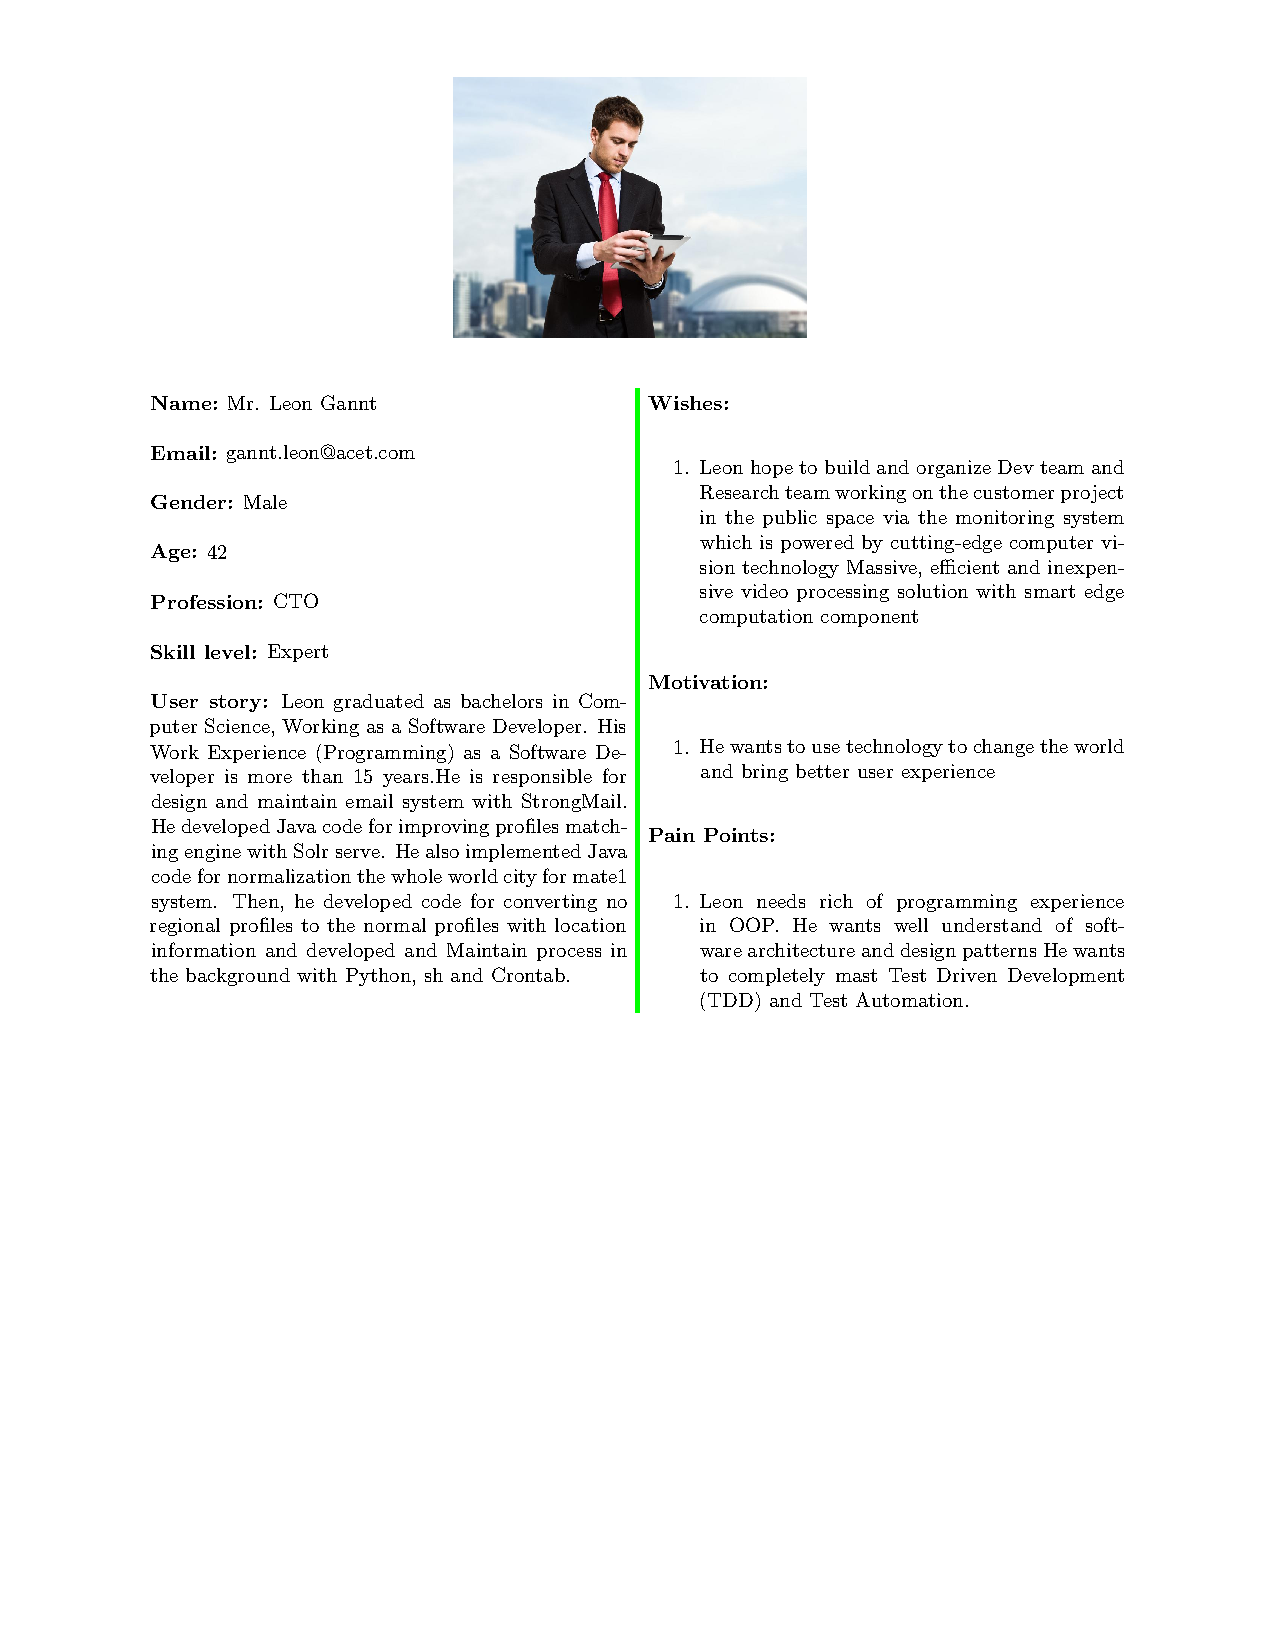
\includepdf[pages=1, scale=1]{images/1.pdf}
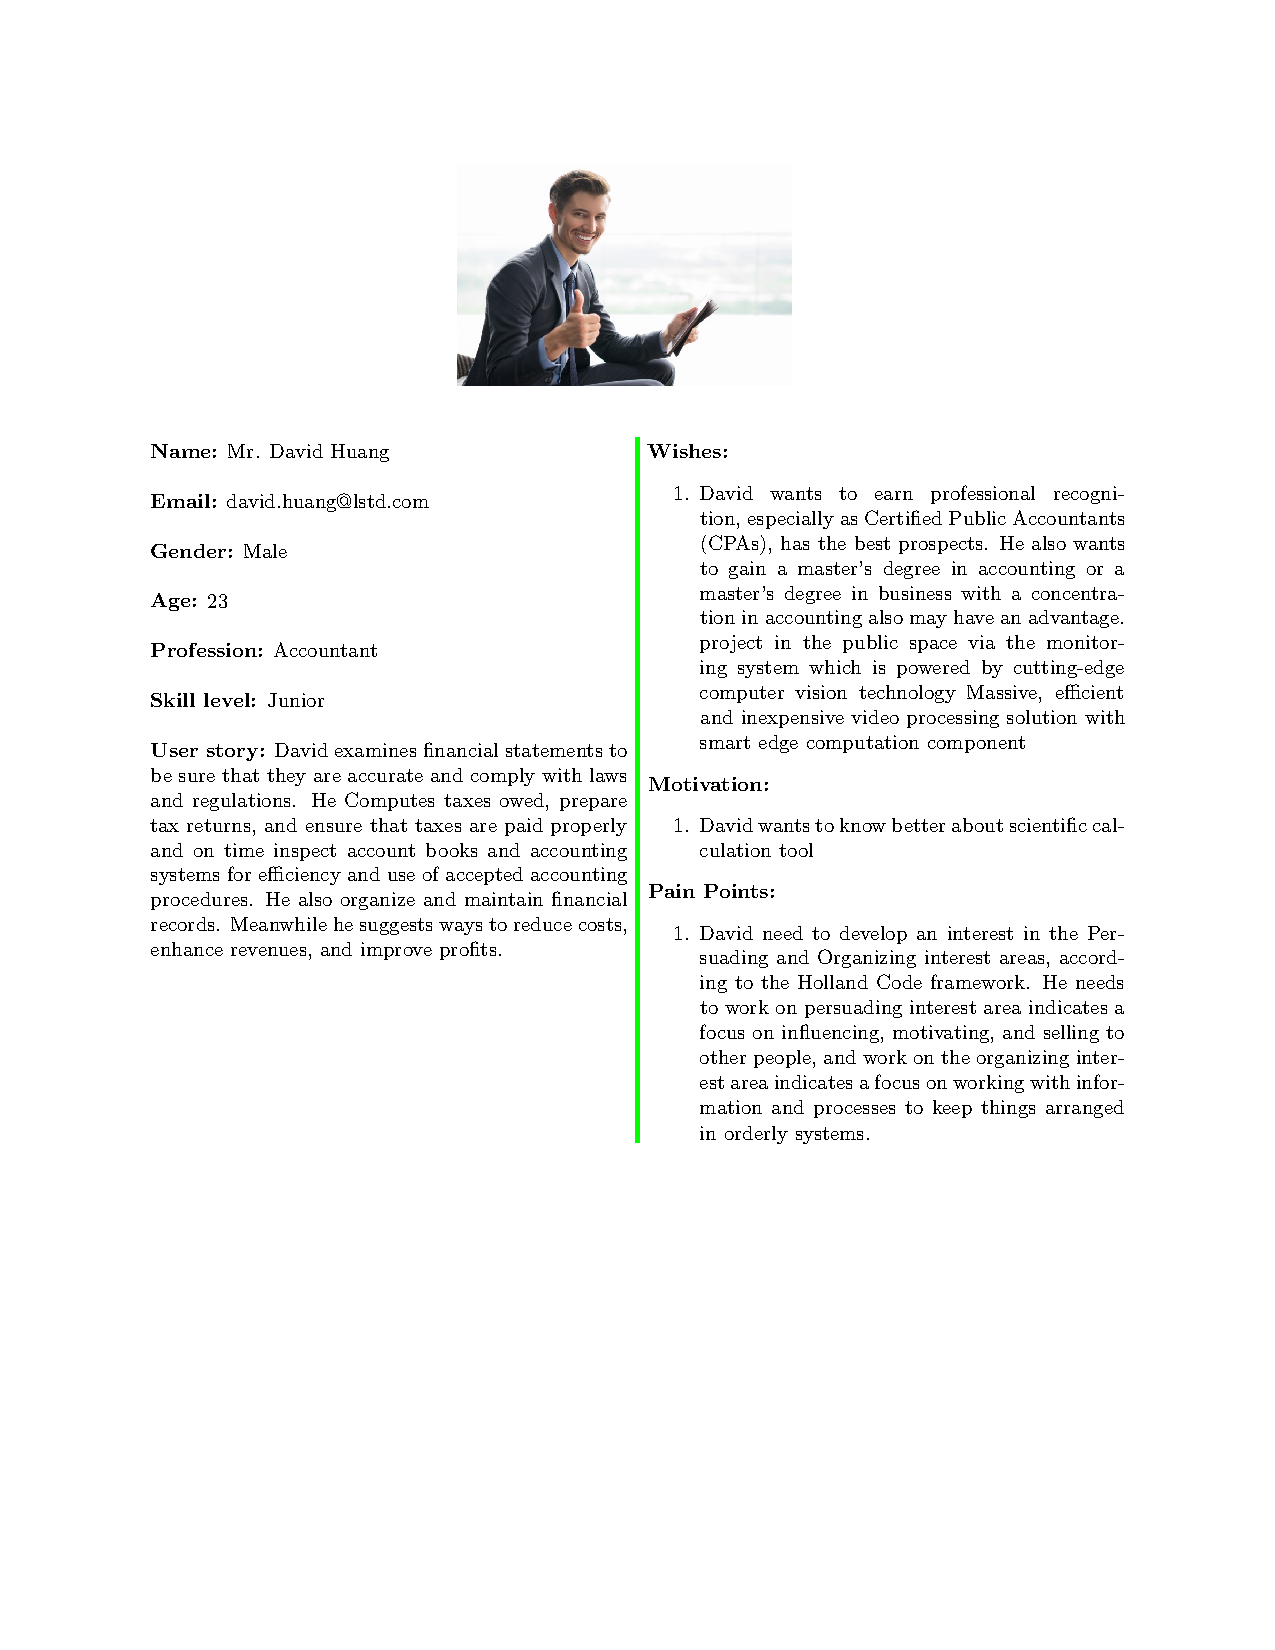
\includepdf[pages=1, scale=1]{images/2.pdf}

% \centering  %图片全局居中
% \includegraphics[width=0.9\linewidth]{images/Persona_1.pdf}


% \section{Junior}
% \centering  %图片全局居中
% \includegraphics[width=0.9\linewidth]{images/Persona_2.pdf}


























